\documentclass{article}
\usepackage{tempora}
\usepackage{indentfirst}
\usepackage{tabularx}
\usepackage{caption}
\usepackage{graphicx}
\usepackage{longtable}
\usepackage{tabularx}
\usepackage{amsmath}
\makeatletter
\renewcommand*\l@section{\@dottedtocline{1}{1.5em}{2.3em}}
\makeatother
\graphicspath{ {./images/} }
\usepackage{float}
\usepackage[english, russian]{babel}

% Ответ должен быть из 2-3х абзацев по 3-4 предложения в каждом
% annakd16@mail.ru - подготовленный документ отправлять сюда
% Дьячук Анна Константиновна

% В 23ем вопросе описать целевую функцию вычисления стоимости для инструментальных средств конфигурирования.

% Описание системы
% 1. Какую систему Вы изучаете в Вашей диссертационной работе? Что является объектом исследования.
% 2. Каково назначение Вашей системы?
% 3. Какова цель исследования системы? Где она может быть использована?
% 4. Частью какой надсистемы является изучаемая система?
% 5. Из каких подсистем состоит система?
% 6. Какие задачи решают подсистемы в составе Вашей системы?
% 7. Сформулируйте кратко сценарий функционирования системы.

% Аспекты внешней среды
% 8. Какие факторы внешней среды Вы учитываете при анализе функционирования системы?
% 9. Какой информацией о факторах внешней среды Вы располагаете (детерминированные, случайные, интервально неопределенные, активное противодействие «противника» или конкурента)?
% 10. Какие показатели эффективности системы в целом и ее подсистем Вы рассматриваете?
% 11. Как в этих показателях учитывается информация о внешней среде?

% Выявление альтернатив системы
% 12. Какое множество альтернатив системы (дискретное, непрерывное, дискретно–непрерывное) Вы рассматриваете?
% 13. Назовите основные структуры и параметры, характеризующие рассматриваемое Вами множество альтернатив системы.
% 14. При каких ограничениях на значения непрерывных параметров системы решается задача?

% Описание модели
% 15. Составьте функциональную схему и опишите функциональные связи между подсистемами в составе системы, а также между подсистемами и внешней средой, которые Вы предполагаете учитывать при разработке математической модели системы.
% 16. Какую систему (или системы) Вы готовы рассматривать как актуальный прототип по отношению к системе, рассматриваемой в Вашей работе?
% 17. Какую задачу – анализа или синтеза системы – Вы решаете? Как решаемая задача связана с целью Вашего исследования?
% 18. Укажите тип математической модели (аналитическая, основанная на использовании физических законов и/или теории, имитационная, эмпирическая), которую Вы будете использовать для решения задачи анализа системы.
% 19. Охарактеризуйте кратко особенности разрабатываемой Вами модели системы.
% 20. В каком состоянии находится разработка модели в настоящее время?
% 21. В какой среде программирования Вы реализуете модель системы?
% 22. Если в работе решается задача синтеза системы, то какой алгоритм оптимизации альтернативы системы Вы используете или предполагаете использовать?
% 23. Если при синтезе системы рассматриваются несколько показателей ее эффективности, то как решается задача оптимизации системы по векторному критерию?

% Заключение
% 24. Какие новые научные и/или практические результаты Вы уже получили (или предполагаете получить) в Вашем исследовании?
% 25. Есть ли у Вас публикации по работе? Выступали ли Вы на научных конференциях по теме Вашей диссертации? Перечислите публикации, укажите место выступления (выступлений).

\begin{document}
    \begin{center}
\textbf{МИНИСТЕРСТВО ОБРАЗОВАНИЯ И НАУКИ РФ}\\[4\baselineskip]
\textbf{Федеральное государственное бюджетное образовательное учреждение высшего образования «Московский авиационный институт (национальный исследовательский университет)»}\\[4\baselineskip]
Институт № 6 «Аэрокосмический» \\[1\baselineskip]
Кафедра 604 «Системный анализ и управление»\\[4\baselineskip]
Реферат\\[2\baselineskip]
На тему: «Исследование и разработка принципов построения инструментальных средств конфигурирования в плагинных системах»\\[1\baselineskip]
По курсу: «Системный анализ»\\[4\baselineskip]
\begin{tabularx}{\textwidth}{ >{\raggedright\arraybackslash}X >{\raggedleft\arraybackslash}X }
    
Выполнил: & Шаблий А.Д. \\
Аспирант группы: & М8О-108А-23 \\
Проверила: & к.т.н. Дьячук А. К. \\
    
\end{tabularx}\\[12\baselineskip]
Москва 2024

\end{center}
    \thispagestyle{empty}
    \newpage

    \tableofcontents
    \thispagestyle{empty}
    \newpage

    \section{Введение}
    В современном мире важную роль в жизни общества занимают информационные технологии. В частности информационные технологии охватывают программные средства, применяемые для цифровых устройств, которые человек использует в повседневной жизни.

Отдельно выделяют класс программных средств - плагинные системы. Это способ организации приложения таким образом, что его конечный объем функционала характеризуется количеством установленных в него расширений - плагинов.

Каждый отдельный плагин включает в себя конечное множество функционала, который в свою очередь основан на требованиях. Именно характер реализованных требований, а так же их объем потребен заказчику. Все остальное - плагины, их взаимосвязи, язык программирования, на котором они реализованы, библиотеки, которые задействованы - все это скрыто от заказчика и зачастую его не интересует. Заказчику интересно, какие свои бытовые или бизнес потребности он сможет удовлетворить от применения программного средства.

На стадии проектирования приложения зачастую неизвестно, какие требования будут востребованы у заказчиков и определить структуру приложения невозможно. Кроме того, для разных заказчиков потребен разный функционал. При необходимости формирования поставки, включающей требуемый объем функционала, поставщик зачастую включает и тот функционал, который не востребован и не оплачен заказчиком, но без которого не быть поставлен востребованный. Это связано с существованием зависимостей у реализации.

Моя диссертационная работа посвящена поиску оптимальной структуры приложения, которая бы с одной стороны позволяла формировать поставки с минимальным числом невостребованного у заказчика функционала, а с другой сдерживала неконтролируемый рост кодовой базы, тем самым, сдерживала стоимость разработки и сопровождения проекта.

    \section{Описание системы}
    % 1. Какую систему Вы изучаете в Вашей диссертационной работе? Что является объектом исследования.
% 2. Каково назначение Вашей системы?
% 3. Какова цель исследования системы? Где она может быть использована?
% 4. Частью какой надсистемы является изучаемая система?
% 5. Из каких подсистем состоит система?
% 6. Какие задачи решают подсистемы в составе Вашей системы?
% 7. Сформулируйте кратко сценарий функционирования системы.

В качесте системы для исследования я обозначил структуру программного средства, предназначенного для интеграции в плагинную систему. Надсистемой является жизненный цикл ПО. Для выявления и описания подсистем мною проанализирована предметная область, сформулированы ограничения на компоненты системы и предложена формулировка ее описания в виде графовой модели. Модель состоит из следующих сущностей, к которым применены ограничения:
\begin{enumerate}
    \item сущности классифицированы:
    \begin{enumerate}
        \item включающая конкретный перечень плагинов поставка;
        \item пригодные для интеграции в плагинную систему плагины;
        \item распределенные по плагинам файлы исходного кода;
        \item функциональные зависимости между файлами исходного кода и плагинами;
        \item реализованные в файлах исходного кода требования.
    \end{enumerate}
    \item один файл исходного кода может реализовывать одно или несколько требований;
    \item одно требование может быть реализовано в одном или нескольких файлах исходного кода;
    \item один файл исходного кода не может быть включен в несколько плагинов;
    \item файлы исходного кода могут иметь зависимости друг на друга, в том числе и циклические;
    \item плагины так же имеют зависимости друг на друга: если в первый плагин включены файлы, зависящие от файлов, расположенных во втором плагине, то первый плагин зависим от второго;
    \item циклические зависимости между плагинами запрещены.
\end{enumerate}

Принципиальная схема приведена на рисунке \ref{fig:graph}.

\begin{figure}[H]
    \centering
    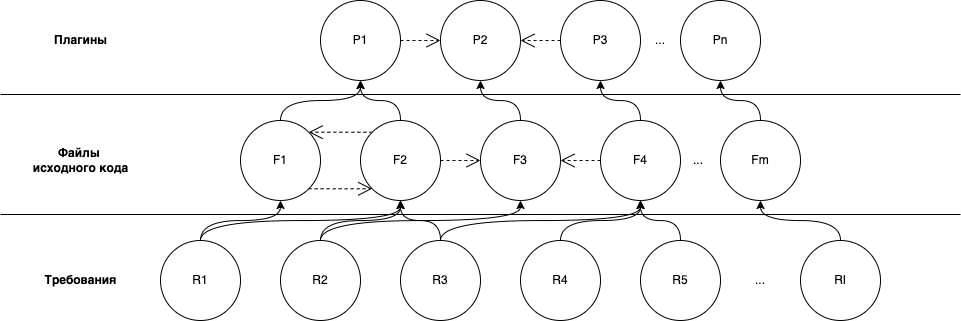
\includegraphics[width=1\textwidth]{graph}
    \caption{Система с приведенными подсистемами}
    \label{fig:graph}
\end{figure}



    \section{Аспекты внешней среды}
    % Аспекты внешней среды
% 8. Какие факторы внешней среды Вы учитываете при анализе функционирования системы?
% 9. Какой информацией о факторах внешней среды Вы располагаете (детерминированные, случайные, интервально неопределенные, активное противодействие «противника» или конкурента)?
% 10. Какие показатели эффективности системы в целом и ее подсистем Вы рассматриваете?
% 11. Как в этих показателях учитывается информация о внешней среде?

Среди аспектов внешней среды системы я выделил изначально сформированный объем требований к системе и требования заказчика, которые могут изменяться от поставки к поставке. От потребных заказчику в рамках поставки объема функционала зависит цена послепродажного обслуживания ПО.

Например, заказчик заказал 10 требований, а поставлен был функционал, реализующий 15. 5 требований он не оплатил, но осуществлять их поддержку все равно необходимо. В данном случае коэффициент простоя равен $5 / 15 = 1/3$. Почти 30\% работы персонала по сопровождению заказчиком не оплачена.

С другой стороны существуют затраты на разработку и поддержку IT продукта. Чем больше в нем сущностей, тем дороже управление его конфигурацией, сложение отношения между сущностями и усложняется поиск и отладка неисправностей. Не говоря уже о когнитивном усложнении восприятии проекта и, как следствие, повышение требований к квалификации разработчиков, что в свою очередь тоже может быть переведено в денежный эквивалент.

Подытоживая, от этих денежных показателей зависит рентабельность IT продукта, а значит и конкурентоспособность бизнеса.

    \section{Выявление альтернатив системы}
    % Выявление альтернатив системы
% 12. Какое множество альтернатив системы (дискретное, непрерывное, дискретно–непрерывное) Вы рассматриваете?
% 13. Назовите основные структуры и параметры, характеризующие рассматриваемое Вами множество альтернатив системы.
% 14. При каких ограничениях на значения непрерывных параметров системы решается задача?
Так какие же варианты? Первое, что следует рассмотреть, как предоставлять заказчику только потребный функционал. Самый очевидный способ реализовать схему 1 требование - 1 плагин. Но этот вариант при достаточно большом объеме требований приведет к неконтролируемому росту сущностей в проекте ПО, следовательно, неконтролируемый рост затрат на его разработку и поддержку. Чтобы их компенсировать производитель будет вынужден повышать цену на свой IT продукт, что снижает конкурентоспособность бизнеса.

Другой альтернативой является схема все требования - 1 плагин. В этом случае коэффициент простоя будет слишком велик, если заказчик заинтересован лишь в части возможностей всего продукта. И службы пост продажного обслуживания будут перегружены, что так же приводит к стоимости поставляемого решения и снижения конкурентоспособности бизнеса.

В своей диссертации я решаю задачу оптимальной декомпозиции функционала по плагинам с целью снижения коэффициента простоя и контроля стоимости разработки и поддержки проекта.

Здесь тоже есть варианты. Первый - декомпозиция по частоте вызова функций. Если функция вызывается редко, она может быть обособлена, чтобы не тянуть свои зависимости в поставку. Часто вызываемые функции напротив, образуют ядро приложения.

Альтернативный - по функциональному признаку. Обосабливать функции по классу решаемых задач. Тогда, если заказчику потребены функции из определенного класса задач, то ему количество функций для решения задач других классов в поставке будет меньше.

    \section{Описание модели}
    % 15. Составьте функциональную схему и опишите функциональные связи между подсистемами в составе системы, а также между подсистемами и внешней средой, которые Вы предполагаете учитывать при разработке математической модели системы.
% 16. Какую систему (или системы) Вы готовы рассматривать как актуальный прототип по отношению к системе, рассматриваемой в Вашей работе?
% 17. Какую задачу – анализа или синтеза системы – Вы решаете? Как решаемая задача связана с целью Вашего исследования?
% 18. Укажите тип математической модели (аналитическая, основанная на использовании физических законов и/или теории, имитационная, эмпирическая), которую Вы будете использовать для решения задачи анализа системы.
% 19. Охарактеризуйте кратко особенности разрабатываемой Вами модели системы.
% 20. В каком состоянии находится разработка модели в настоящее время?
% 21. В какой среде программирования Вы реализуете модель системы?
% 22. Если в работе решается задача синтеза системы, то какой алгоритм оптимизации альтернативы системы Вы используете или предполагаете использовать?
% 23. Если при синтезе системы рассматриваются несколько показателей ее эффективности, то как решается задача оптимизации системы по векторному критерию?

Попытки описания механизмов, позволяющих реализовать разделение функционала уже существуют в наше время. Примером является Equenox - реализация спецификации OSGI, которая лежит в основе IDE Eclipse.

Спецификация OSGI предполагает построение (синтез) системы из обособленных компонентов. Для разделения зависимостей на сторонние библиотеки и сервисы. Степень разделения и ее характер зависит от реализации. В IDE Eclipse она реализована для решения целей и задач стоящих перед самой IDE, однако предполагает ее расширение по правилам конкретного бизнеса.

В рамках диссертационного иссследования, следуя правилам спецификации OSGI, мною на языке программирования Java написано решение подзадачи изменения исходного графа с учетом разрешения циклических зависимостей между файлами исходного кода. В решении получены результаты экспериментов для оценки времени работы приложения от типа используемых коллекций, в которых хранится информация о графе:
\begin{enumerate}
    \item вершины - файлы исходного кода и требования к ПО;
    \item ребра - зависимости между файлами исходного кода и трассируемость требований к ПО.
\end{enumerate}

Работа алгоритма заключается в итеративном поиске циклов в графе с последующим слиянием входящем в цикл вершин до тех пор, пока в графе не будут отсутствовать циклы.

Схема разработанного решения приведена на рисунке \ref{fig:application_scheme}.

\begin{figure}[H]
    \centering
    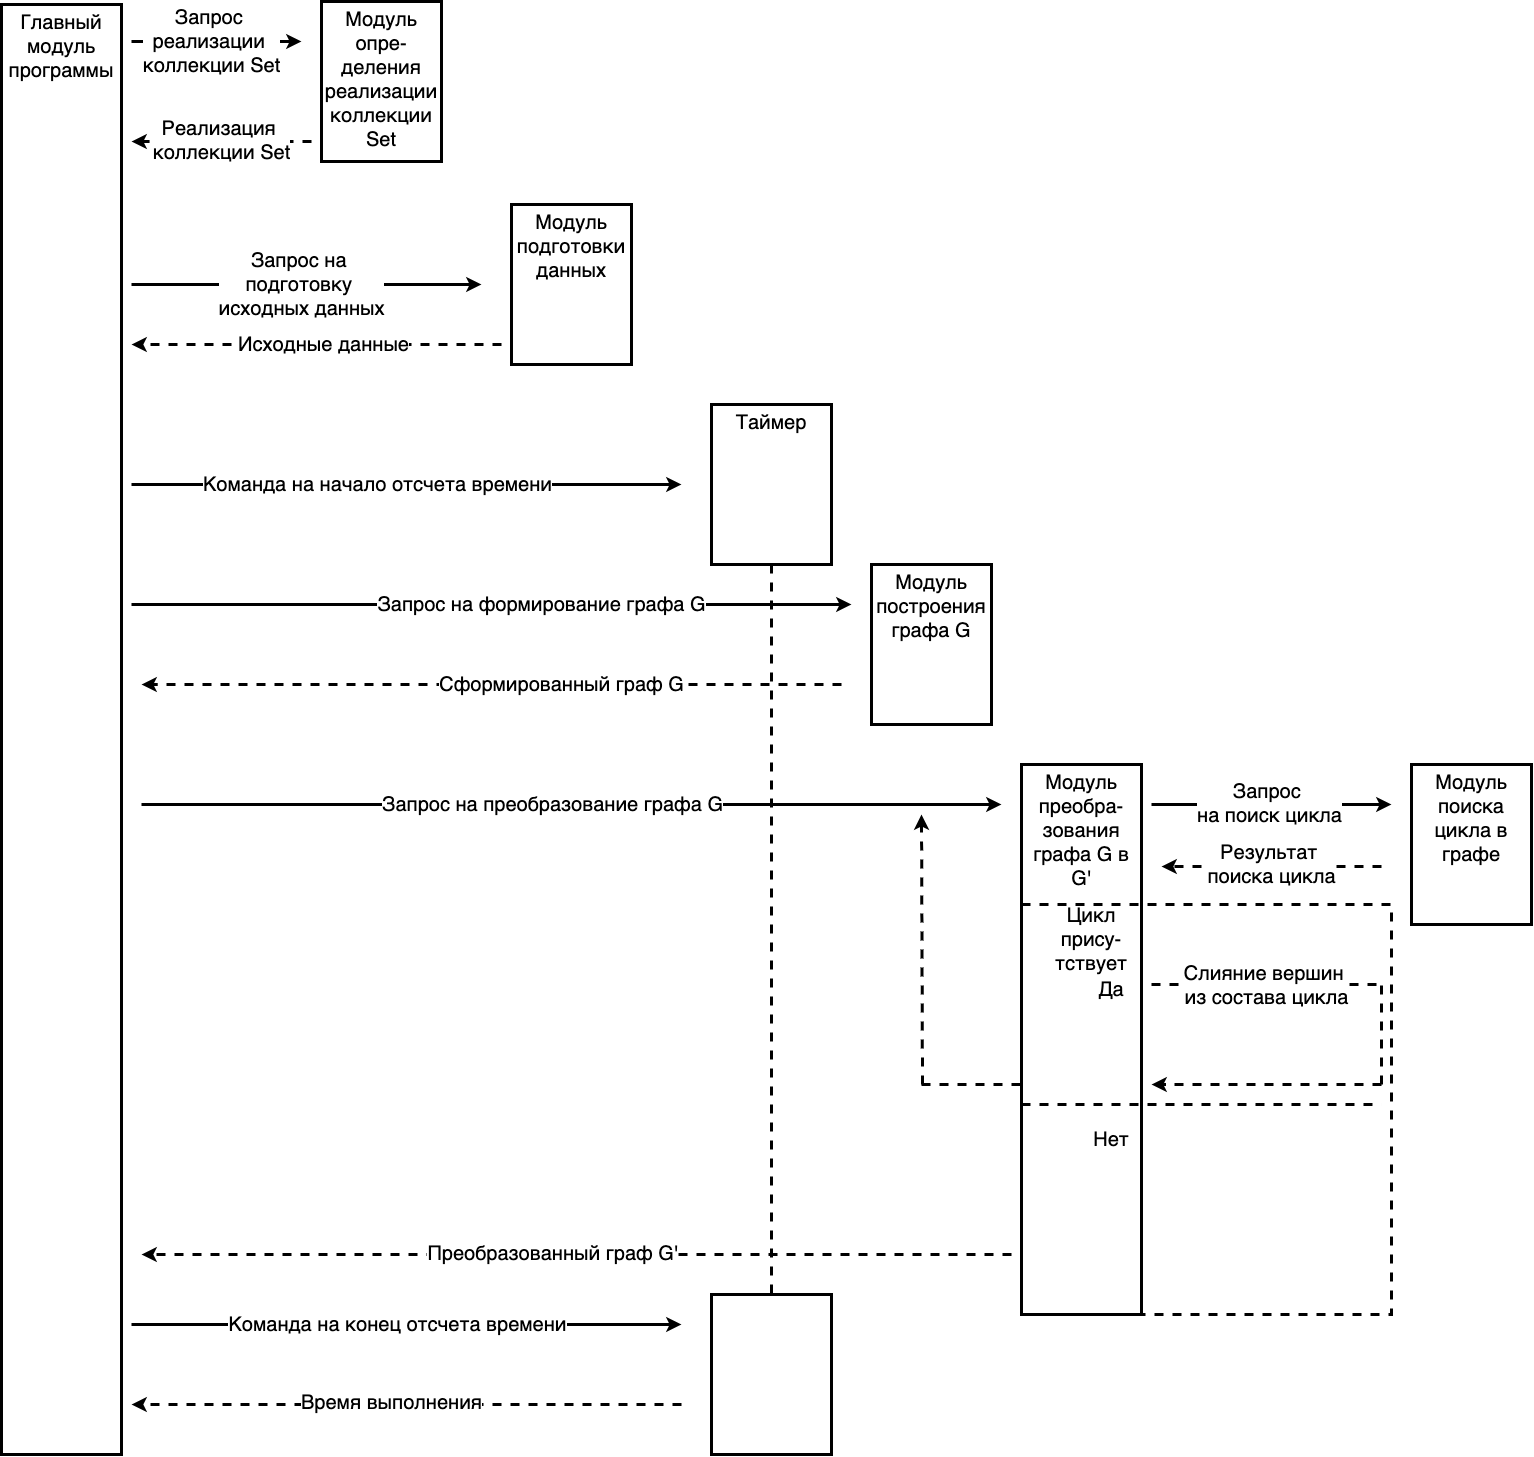
\includegraphics[width=1\textwidth]{application_scheme}
    \caption{Схема разработанного решения}
    \label{fig:application_scheme}
\end{figure}

В дальнейшем предполагается доработка модели для поиска оптимального распределения файлов исходного кода по плагинам.

Для выявления лучшего решения сформулирован векторный критерий:
\begin{enumerate}
    \item возможность динамеческого ценнобразования поставки $C_{d}$;
    \item $V_{c}$;
    \item $K_{f}$;
\end{enumerate}

% Рассказать про каждый коэффициент, какой диапазон значений принимает
$C_{d}$ является определяющим фактором. Именно благодара ему достигается динамическое изменение $K_{f}$ при статических $R^{*}$ и $V_{c}$.

$ C_{d} =
  \begin{cases}
    1 & \quad \text{если } R^{*} \not = R^{*}_{d}\\
    0 & \quad \text{если } R^{*} = R^{*}_{d}\\
  \end{cases}
$

$V_{c}$ определяет общий объем кодовой базы, поддержку которого необходимо осуществлять. Чем больше объем, тем более дорогой является поддержка.

$ V_{c} =
  \begin{cases}
    1 & \quad \text{если } N_{p} = 1 \\
    2 & \quad \text{если } 1 < N_{p} < N_{f} \\
    3 & \quad \text{если } N_{p} = N_{f}
  \end{cases}
$

$K_{f}$ не статичен и может быть уникален для каждой из поставок.

Так, вектора показателей эффективности для сформулированных альтернати в предлагаемого решения следующие:
\begin{enumerate}
    \item альтернатива по схеме <<1 требование - 1 файл исходного кода - 1 плагин>>:
    \begin{itemize}
        \item $C_{d} = 1$;
        \item $V_{c} = 3$;
        \item $K_{f} = 0$.
    \end{itemize}
    \item альтернатива по схеме <<все требования - 1 плагин>>:
    \begin{itemize}
        \item $C_{d} = 0$;
        \item $V_{c} = 1$;
        \item $K_{f} \approx 1$.
    \end{itemize}
    \item предлагаемое решение:
    \begin{itemize}
        \item $C_{d} = 1$;
        \item $V_{c} = 2$;
        \item $0 < K_{f} < 1$.
    \end{itemize}
\end{enumerate}

В предлагаемом решении $C_{d}$ = 1, что обеспечивает главное условие - динамическое изменение $K_{f}$ при статических $R^{*}$ и $V_{c}$. Несмотря на увеличение $V_{c}$ по сравнению со схемой <<все требования - 1 плагин>>, $V_{c}$ не увеличивается на столько как в схеме <<1 требование - 1 файл исходного кода - 1 плагин>>. Применяя различные алгоритмы оптимизации, приследуется цель выявления такой декомпозиции, которая обеспечивала бы минимизацию значения $K_{f}$. Предполагается использовать следующие алгоритмы оптимизации:
\begin{enumerate}
    \item генетический алгоритм;
    \item PageRank;
    \item решающий лес.
\end{enumerate}

    \section{Заключение}
    % Заключение
% 24. Какие новые научные и/или практические результаты Вы уже получили (или предполагаете получить) в Вашем исследовании?
% 25. Есть ли у Вас публикации по работе? Выступали ли Вы на научных конференциях по теме Вашей диссертации? Перечислите публикации, укажите место выступления (выступлений).

В заключении хочу сказать, что полученные мною результаты применяются для различных приложений и решений выполненных как набор плагинов для интеграции в соответствующие им плагинные системы.

Так, на конференции в МГТУ им. Баумана я в своем докладе «Исследование правил построения конфигуратора ARINC 653 спецификации в IDE Eclipse» показал результаты применения сформулированной модели для решения задачи по критерию частот вызова функций. В качестве результата продемонстрировал снижение невостребованного функционала до 10\% при различных запросах состава требований.

На конференции в Воронеже в ВУНЦ ВВС «ВВА имени профессора Н.Е. Жуковского и Ю.А. Гагарина» в своем докладе «Реализация инструментального средства конфигурирования компонентов БРЭО» показал актуальность применения плагинных систем для решения задач в авиационной сфере.

Подготовил выступление на конференции, организуемой Союзом Машиностроителей России, в качестве материала выступления мною предоставлено средство интеллектуального конфигурирования системы определения состояния воздушного судна. В этой работе я сформировал среду конфигурирования, которая независимо подключается к базе данных и заполняет ее конфигурационными параметрами и их значениями с целью дельнейшей их обработки непосредственно в самой системе.

Подготовлена публикация ВАК, в которой описан алгоритм разрешения циклических зависимостей графовой модели трассируемости требований к ПО на файлы исходного кода. Работа передана в редакцию ИПМ им. М.В.Келдыша РАН.

\end{document}